\documentclass[
	aspectratio=169, % default is 43
	8pt, % font size, default is 11pt
	handout, % handout mode without animations, comment out to add animations
]{beamer}
\def\university{magdeburg}

\documentclass[
	aspectratio=169, % default is 43
	8pt, % font size, default is 11pt
	handout, % handout mode without animations, comment out to add animations
]{beamer}

\usepackage{../template/beamerthemeuulm} % use the inofficial uulm beamer theme
\setfaculty{infIngPsy} % set the color scheme for your faculty here [med/infIngPsy/math/nat]

% requires symbolic links
% git clone git@github.com:SoftVarE-Group/SlideTemplate.git C:\Users\...\SlideTemplate
% mklink /J template C:\Users\...\SlideTemplate
% git clone git@spgit.informatik.uni-ulm.de:thuem/slides.git C:\Users\...\ThomasSlides
% mklink /J thomasslides C:\Users\...\ThomasSlides
\graphicspath{{../template/pics/logos}{../template/pics/nature}{../template/pics/uulm}{../thomasslides/}{../pics/people/}{../pics/xkcd/}}

%\usepackage[ngerman]{babel} % use this line for slides in German
%\recordingtrue % special recording mode for use with a greenscreen, gives you space to show yourself in a layer in front of the slides, has no effect in the handout mode

\title{Software Product Lines} % short title is used for the slide footer but optional

% LINKED LITERATURE

\newcommand{\ludewiglichter}{\href{https://learning.oreilly.com/library/view/-/9781457184932/?ar}{Ludewig and Lichter}}
\newcommand{\seeconomics}{\href{https://rds-ulm.ibs-bw.de/link?kid=027381854}{SE Economics}}
\newcommand{\sommervillelink}[1]{\href{https://ulm.ibs-bw.de/aDISWeb/app?service=direct/0/Home/$DirectLink\&sp=SOPAC00\&sp=SAKSWB-IdNr1615420983}{#1}}
\newcommand{\sommerville}{\sommervillelink{Sommerville}}
\newcommand{\thehumbleprogrammer}{\href{https://dl.acm.org/doi/10.1145/1283920.1283927}{The Humble Programmer}}
\newcommand{\thepragmaticprogrammer}{\href{https://learning.oreilly.com/library/view/the-pragmatic-programmer/9780135956977/}{The Pragmatic Programmer}}

% TYPICAL COMMANDS FOR LECTURES

\renewcommand{\emph}[1]{{\color{blue}\textbf{#1}}}

\newcommand{\deutsch}[1]{{\color{blue}(#1)}}
\newcommand{\deutschertitel}[1]{{\tiny\deutsch{#1}}}

\newcommand{\mycite}[1]{``#1''}
\newcommand{\mytitlesource}[1]{{\tiny\normalfont\mbox{[#1]}}}
\newcommand{\mysource}[1]{\ifthenelse{\equal{#1}{}}{}{\phantom{.}~\hfill~\mytitlesource{#1}}}

\newcommand{\todo}[1]{{\color{red}\textbf{[#1]}}}
\newcommand{\fodo}[1]{\todo{\footnote{\todo{#1}}}}
\newcommand{\todots}{\todo{\ldots}}

% IMPORTED PACKAGES

%\usepackage{adjustbox} % used for partofpage
%\usepackage{tcolorbox} % used for mydefinition, mynote, myexample
\usepackage{multicol} % used temporarily for the lecture overview
\usepackage{mathtools} % required for absolute value in modeling lecture

% COMMANDS TO LAYOUT AND ANNIMATE SLIDES

\newcommand{\lessonslearned}[3]{
	\subsection{Summary}
	\begin{frame}{\insertsection -- \insertsubsection}
		\leftorright{
			\mydefinition{Lessons Learned}{
				\begin{itemize}
					#1
				\end{itemize}
			}
			\mynote{Further Reading}{
				\small % references take space, can be a little smaller
				\begin{itemize}
					#2
				\end{itemize}
			}
		}{
			\myexample{Practice}{
				#3
			}
		}
	\end{frame}
}

% TODO temporary hack to layout the slide overview in two colums
\renewcommand{\lectureoverview}{
%	\section*{Overview}
%	\subsection*{Overview}
	\begin{frame}{\insertsubtitle}
		\begin{multicols}{2}
			\tableofcontents
		\end{multicols}
	\end{frame}
}

\renewcommandx{\maketitle}[2][1=apr21-o25a,2=150]{
    {
	\usebackgroundtemplate{} % TODO temporary hack to enable missing pictures at title slide
	%\ifx {#1} \empty \else {\usebackgroundtemplate{\includegraphics[trim=0 0 0 #2,clip,width=\paperwidth]{#1}}} \fi     
	%\usebackgroundtemplate{\includegraphics[trim=0 0 0 #2,clip,width=\paperwidth]{#1}}
    \begin{frame}[plain]
        \vskip0pt plus 1filll
        \begin{beamercolorbox}[wd=\paperwidth,ht=4.5ex,dp=2ex,right]{titlebox}
            \LARGE\textbf{\inserttitle}\hspace*{20pt}
        \end{beamercolorbox}%
        \nointerlineskip%
        \begin{beamercolorbox}[wd=\paperwidth,ht=2.25ex,dp=1ex,right]{subtitlebox}
            \small 
            \ifx \insertsubtitle \empty \else \insertsubtitle\ $\vert$ \fi
            \insertauthor\
            \ifx \insertdate \empty \else $\vert$ \insertdate \fi
            \hspace*{20pt}
        \end{beamercolorbox}%
        \nointerlineskip%
        \begin{beamercolorbox}[wd=\paperwidth,ht=4.5ex,dp=2ex,left]{logobox}
            \centering
            \vspace{-1ex}
            \hspace{10pt}
            \includegraphics[height=4.5ex]{sp} % SPECIFY INSTITUTE LOGO HERE
            \hfill
            \includegraphics[height=4.5ex]{uulm}
            \hspace{10pt}
        \end{beamercolorbox}%
    \end{frame}
    }  
}

%
%\newcommand{\onlyleft}[1]{
%	\halfpage{#1}
%}
%
%\newcommand{\onlyright}[1]{
%	~\hfill
%	\halfpage{#1}
%}
%
%\newcommand{\leftorright}[2]{
%	\uncover<1>{\halfpage{#1}}
%	\hfill
%	\uncover<3->{\halfpage{#2}}
%}
%
%\newcommand{\rightorleft}[2]{
%	\uncover<3->{\halfpage{#1}}
%	\hfill
%	\uncover<1>{\halfpage{#2}}
%}
%
%\newcommand{\leftthenright}[2]{
%	\halfpage{#1}
%	\hfill\pause
%	\halfpage{#2}
%}
%
%\newcommand{\leftandright}[2]{
%	\halfpage{#1}
%	\hfill
%	\halfpage{#2}
%}
%
%\newcommand{\leftmiddleandright}[3]{
%	\thirdpage{#1}
%	\hfill
%	\thirdpage{#2}
%	\hfill
%	\thirdpage{#3}
%}
%
%\newcommand{\leftmiddleorright}[3]{
%	\uncover<1>{\thirdpage{#1}}
%	\hfill
%	\uncover<3>{\thirdpage{#2}}
%	\hfill
%	\uncover<5->{\thirdpage{#3}}
%}
%
%\newcommand{\halfpage}[1]{\partofpage{48}{#1}}
%
%\newcommand{\thirdpage}[1]{\partofpage{31}{#1}}
%
%\newcommand{\partofpage}[2]{
%	\adjustbox{valign=t}{\begin{minipage}{0.#1\textwidth}
%			\begin{flushleft}
%				#2
%			\end{flushleft}
%	\end{minipage}}
%}
%
%\newcommand{\mydefinition}[2]{
%	\begin{tcolorbox}[title=#1,colback=orange!10,colframe=orange!30,coltitle=black,fonttitle=\bfseries,left=1mm,right=1mm,top=1mm,bottom=1mm]
%		\begin{flushleft}
%			#2
%		\end{flushleft}
%	\end{tcolorbox}
%}
%
%\newcommand{\mydefinitiontight}[2]{
%	\begin{tcolorbox}[title=#1,colback=white,colframe=orange!30,coltitle=black,fonttitle=\bfseries,left=0mm,right=0mm,top=0mm,bottom=0mm]
%		\begin{flushleft}
%			#2
%		\end{flushleft}
%	\end{tcolorbox}
%}
%
%\newcommand{\mynote}[2]{
%	\begin{tcolorbox}[title=#1,colback=red!10,colframe=red!30,coltitle=black,fonttitle=\bfseries,left=1mm,right=1mm,top=1mm,bottom=1mm]
%		\begin{flushleft}
%			#2
%		\end{flushleft}
%	\end{tcolorbox}
%}
%
%\newcommand{\myexample}[2]{
%	\begin{tcolorbox}[title=#1,colback=blue!10,colframe=blue!30,coltitle=black,fonttitle=\bfseries,left=1mm,right=1mm,top=1mm,bottom=1mm]
%		\begin{flushleft}
%			#2
%		\end{flushleft}
%	\end{tcolorbox}
%}
%
%\newcommand{\myexampletight}[2]{
%	\begin{tcolorbox}[title=#1,colback=white,colframe=blue!30,coltitle=black,fonttitle=\bfseries,left=0mm,right=0mm,top=0mm,bottom=0mm]
%		\begin{flushleft}
%			#2
%		\end{flushleft}
%	\end{tcolorbox}
%}

\subtitle{4. Feature Modeling}
\author{Elias Kuiter, Thomas Thüm, Timo Kehrer}
\foruniversity{}
	{\setpicture[50]{ovgu-autumn3}\setcopyright{Photo: Hannah Theile (OVGU)}}
	{\setpicture{oct20-south4}}

\begin{document}

\mode<handout>{\contentoverview}

\mode<beamer>{
	\ifdefined\thepicture
		\maketitle[\thepicture][\thepictureoffset]
	\else
		\maketitle[]
	\fi
}

% shared slide content

% introduced: 02a-configuration
% reused: 03a-intro
\newcommand{\frameImplementSPLs}{
	\begin{mycolumns}[widths={45},animation=none]
		\pic[width=\linewidth]{metaproduct2}
	\mynextcolumn
		\begin{note}{Key Issues}
			\begin{itemize}
			\item Systematic reuse of implementation artifacts
			\item Explicit handling of variability
			\end{itemize}
		\end{note}
		\uncover<2->{\begin{definition}{Variability\mysource{\fospl\mypage{48}}}
			\mycite{\emph{Variability} is the ability to derive different products from a common set of artifacts.}
		\end{definition}}
		~
		\uncover<3->{\begin{note}{Variability-Intensive System}
			Any software product line is a variability-intensive system. % TODO Timo: do we really need this term? where does this definition come from?
		\end{note}}
	\end{mycolumns}
}

% introduced: 02a-configuration
% reused: 02b-implementation, 03a-intro
\newcommand{\frameVariabilityAndBindingTimes}{
	\begin{mycolumns}[widths={55},animation=none]
		\begin{definition}{Binding Time \deutsch{Bindungszeitpunkt}\mysource{\fospl\mypage{48}}}
			\begin{itemize}
				\item Variability offers choices
				\item Derivation of a product requires to make decisions (aka. binding)
				\item Decisions may be bound at different binding times
			\end{itemize}
		\end{definition}
		~
		\uncover<2->{\begin{note}{When? By whom? How?}
			\lectureruntime\parta: \emph{when} and \emph{by whom}

			\lectureruntime\partb: \emph{how}
		\end{note}}
	\mynextcolumn
		\pic[width=\linewidth]{metaproduct2}
	\end{mycolumns}
}

% introduced: 03a-intro
% reused: 03a-intro
\newcommand{\frameRuntimeVariabilityProblems}{
	\begin{note}{Problems of Runtime Variability}
		{\bf Conditional Statements:}
		\begin{itemize}
			\item Code scattering, tangling, and replication
		\end{itemize}
		{\bf Design Patterns for Variability:}
		\begin{itemize}
			\item Trade-offs and potential negative side effects
			\item Constraints that may restrict their usage
		\end{itemize}
		{\bf In General:}
		\begin{itemize}
			\item Variable parts are always delivered
			\item Not well-suited for compile-time binding
		\end{itemize}
	\end{note}
}

% introduced: 03a-intro
% reused: 03a-intro
\newcommand{\frameSoftwareConfigurationManagement}{
	\begin{mycolumns}
		\begin{definition}{Software Configuration Management} % TODO source missing
			Policies, processes, and tools for managing evolving software systems:
			\begin{itemize}
				\item Version control
				\item System building
				\item Release management
				\item Change management
				\item Collaborative work
			\end{itemize}
		\end{definition}
	\mynextcolumn
		\begin{note}{No Software Configuration Management}
			\lecturecloneandown\parta: Ad-Hoc Clone-and-Own

			aka.\ unmanaged clone-and-own
		\end{note}
		\begin{note}{Version Control}
			\lecturecloneandown\partb: Clone-and-Own with Version Control

			instance of managed clone-and-own
		\end{note}
		\begin{note}{System Building}
			\lecturecloneandown\partc: Clone-and-Own with Build Systems

			instance of managed clone-and-own
		\end{note}
	\end{mycolumns}
}


\section{Feature Models}

\subsection{Recap: Software Product Lines}
\begin{frame}{\myframetitle\ \mytitlesource{\lectureintroduction}}
	\begin{mycolumns}[t]
		\begin{definition}{Software Product Line \mysource{\seiwhitepaperspl\mypage{5}}}
			\mycitebegin A \emph{software product line} is 
			\begin{itemize}
				\item a set of software-intensive systems
				\item that share a common, managed set of features
				\item satisfying the specific needs of a particular market segment or mission
				\item and that are developed from a common set of core assets in a prescribed way.\myciteend
				\mysource{\href{https://resources.sei.cmu.edu/library/asset-view.cfm?assetID=513819}{Software Engineering Institute, Carnegie Mellon University}}
			\end{itemize}
		\end{definition}
		\begin{definition}{Product \mysource{\fospl\mypage{19}}}
			\mycite{A \emph{product of a product line} is specified by a valid feature selection (a subset of the features of the product line). A feature selection is \emph{valid} if and only if it fulfills all feature dependencies.}
		\end{definition}
	\mynextcolumn
		\begin{definition}{Feature \mysource{\fospl\mypage{18}}}
			\mycite{A \emph{feature} is a characteristic or end-user-visible behavior of a software system.}
		\end{definition}
		\centering\xkcd{2369}{width=.9\linewidth,trim=35 35 35 35,clip}
	\end{mycolumns}
\end{frame}

\subsection{Features Have Dependencies}

\begin{frame}{\myframetitle}
	\begin{mycolumns}[columns=3,widths={40,20,40}]
		\myexampletight{Ordering a Waffle \ldots}{
			\pic[width=\textwidth]{waffle-feature-model}
		}
		\mynextcolumn
		\myexampletight{\ldots with Sugar}{
			\pic[width=\textwidth]{waffle-sugar}
		}
		\myexampletight{\ldots with Cherries}{
			\pic[width=\textwidth]{waffle-cherries}
		}
		\mynextcolumn
		\begin{note}{This is Nice, But \ldots}
			\begin{itemize}
				\item plate and sugar seem to always be included, a fork is only included for some orders\\
					$\Rightarrow$ limitations seem \emph{arbitrary}
				\item children get special treatment\\
					$\Rightarrow$ order process is \emph{unfair}
				\item what exactly am I paying for?\\
					$\Rightarrow$ investments are \emph{unclear}
			\end{itemize}
		\end{note}
		\begin{definition}{In This Lecture}
			\begin{enumerate}
				\item how to \emph{model and configure} features and their dependencies?
				\item how to \emph{store and communicate}?
				\item how to \emph{analyze and understand}?
			\end{enumerate}
		\end{definition}
	\end{mycolumns}
\end{frame}

\subsection{Specifying Valid Configurations}

\newcommand{\feat}[1]{{\emph{#1}}}
\newcommand{\exampleFeatureSetConfigDB}{
	\vspace*{-4ex}
	\begin{align*}
		\text{Feature set } F = \{&\textbf{C}onfigDB, \textbf{G}et, \textbf{P}ut, \textbf{D}elete,\\
		&\textbf{T}ransactions, \textbf{W}indows, \textbf{L}inux\}
	\end{align*}
}

\begin{frame}{\myframetitle}
	\begin{mycolumns}
		\begin{definition}{Configuration}
			\begin{itemize}
				\item a \emph{configuration} \deutsch{Konfiguration} over a set of features $F$ selects and deselects features in $F$
				\item formally: a pair $(S, D)$ such that $S, D \subseteq F$ and $S, D$ are disjoint ($S \cap D = \varnothing$)
				\item is \emph{complete} \deutsch{vollständig} if all features are covered ($S \cup D = F$) and \emph{partial} \deutsch{partiell} otherwise
				\item a complete configuration is \emph{valid} \deutsch{gültig} if it ``makes sense'' in the domain and \emph{invalid} \deutsch{ungültig} otherwise % TODO why only complete configurations? probably easier to understand here, but validity could also be useful for partial configurations later
				\item we often abbreviate complete configurations with $S \equiv (S, F \setminus S)$
			\end{itemize}
		\end{definition}
	\mynextcolumn
		\myexample{}{
			\exampleFeatureSetConfigDB
			Examples for \emph{complete} configurations:
			\begin{itemize}
				\item \emph{valid} (read-only database on Windows):
					$\cfg{C, G, W}{P, D, T, L}$
				\item \emph{valid} (fully functional database on Linux):
					$\cfg{C, G, P, D, T, L}{W}$
				\item \emph{invalid} ($\lightning$ no operating system):
					$\cfg{C, G}{P, D, T, W, L}$
				\item \emph{invalid} (transactions $\lightning$ read-only database):
					$\cfg{C, G, T, L}{P, D, W}$
			\end{itemize}
			Examples for \emph{partial} configurations:
			
			$\cfg{C, G}{P, D}$, $(\varnothing, \varnothing)$
		}
	\end{mycolumns}
\end{frame}

\subsubsection{Natural Language}

\begin{frame}{\myframetitle}\label{frame:natlang}
	\begin{mycolumns}
		\begin{note}{Valid Configuration}
			A complete configuration over $F$ is valid if it ``makes sense'' in the domain.
			\emph{\color{red}{$\leadsto$ ``makes sense''?}}
		\end{note}

		\begin{definition}{Natural Language}
			\begin{itemize}
				\item informal description of relationships between features in $F$
				\item a complete configuration $S$ is \emph{valid} if it conforms to the description
				\item[+] succinct
				\item[--] sometimes ambiguous
				\item[--] not machine-readable
			\end{itemize}
		\end{definition}
	\mynextcolumn
		\myexample{}{
			``A \feat{configurable database} has an API that allows for at least one of the request types \feat{Get}, \feat{Put}, or \feat{Delete}.
			Optionally, the database can support \feat{transactions}, provided that the API allows for Put or Delete requests.
			Also, the database targets a supported operating system, which is either \feat{Windows} or \feat{Linux}.''
		}
	\end{mycolumns}
\end{frame}

\subsubsection{Configuration Map}

\begin{frame}{\myframetitle}\label{frame:cfgmap}
	\begin{mycolumns}
		\begin{note}{Valid Configuration}
			A complete configuration over $F$ is valid if it ``makes sense'' in the domain.
			\emph{\color{red}{$\leadsto$ ``makes sense''?}}
		\end{note}

		\begin{definition}{Configuration Map}
			\begin{itemize}
				\item a \emph{configuration map} over $F$ is a set of complete configurations $M \subseteq \power{F}$
				\item a complete configuration $S$ is \emph{valid} if it occurs in the configuration map ($S \in M$)
				\item also known as product map
				\item[+] precise
				\item[--] not human-readable
				\item[--] redundant, explodes in size ($0 \leq \abs{M} \leq 2^{\abs{F}}$)
			\end{itemize}
		\end{definition}
	\mynextcolumn
		\myexample{}{
			\exampleFeatureSetConfigDB
			Configuration map:\\\small
			\begin{mycolumns}[animation=none]
				{\color{black}$\{C,G,W\}$}\\
				$\{C,P,W\}$\\
				$\{C,G,P,W\}$\\
				$\{C,D,W\}$\\
				$\{C,G,D,W\}$\\
				$\{C,P,D,W\}$\\
				$\{C,G,P,D,W\}$\\
				$\{C,P,T,W\}$\\
				$\{C,G,P,T,W\}$\\
				$\{C,D,T,W\}$\\
				$\{C,G,D,T,W\}$\\
				$\{C,P,D,T,W\}$\\
				$\{C,G,P,D,T,W\}$
			\mynextcolumn
				$\{C,G,L\}$\\
				$\{C,P,L\}$\\
				$\{C,G,P,L\}$\\
				$\{C,D,L\}$\\
				$\{C,G,D,L\}$\\
				$\{C,P,D,L\}$\\
				$\{C,G,P,D,L\}$\\
				$\{C,P,T,L\}$\\
				$\{C,G,P,T,L\}$\\
				$\{C,D,T,L\}$\\
				$\{C,G,D,T,L\}$\\
				$\{C,P,D,T,L\}$\\
				{\color{black}$\{C,G,P,D,T,L\}$}
			\end{mycolumns}
		}
	\end{mycolumns}
\end{frame}

\subsubsection*{Configuration Map in Excel}

\begin{frame}{\myframetitle}
	\centering
	\picDark[width=0.48\linewidth]{products-in-excel}

	\textbf{Can we do better?}
\end{frame}

\subsection{Feature Models}

\subsubsection*{Syntax}

\begin{frame}{\myframetitle\ \mytitlesource{\fospl; \foda\mypages{63--72}; \batorygrammars}}
	\begin{mycolumns}
		\centering
		\featureDiagramConfigurableDatabase
		
		\featureDiagramLegend
	\mynextcolumn
		\begin{definition}{Feature Model \deutsch{Feature-Modell}}
			\begin{itemize}
				\item hierarchy of features
				\item dependencies between features modeled by tree and cross-tree constraints
				\item \emph{tree constraints}: defined by the hierarchy
				\item \emph{cross-tree constraints}: propositional formulas over features
				\item \emph{abstract features} are used to group other features
				\item \emph{concrete features} have an implementation
				\item also known as feature diagram or feature tree
				\item notation for \emph{optional/mandatory features} and \emph{or/alternative groups}
			\end{itemize}
		\end{definition}
	\end{mycolumns}
\end{frame}

\subsubsection*{Semantics}

\begin{frame}{\myframetitle\ \mytitlesource{\fospl; \batorygrammars}}
	\begin{mycolumns}[animation=none]
		\uncover<2-|handout:1>{
			\begin{definition}{Tree Constraints}
				\begin{itemize}
					\item the \emph{root feature} is always required
					\item each feature requires its parent (aka.~\emph{parent-child-relationship})
					\item an \emph{optional feature} can be (de-)selected freely when its parent is selected
					\item a \emph{mandatory feature} is required by its parent
					\item \emph{or group}: at least one child feature must be selected when the parent is selected
					\item \emph{alternative group}: exactly one child feature must be selected when the parent is selected
				\end{itemize}
			\end{definition}
		}
	\mynextcolumn
		\centering
		\featureDiagramConfigurableDatabase
		\uncover<3|handout:1>{
			\begin{definition}{Cross-Tree Constraints}
				\begin{itemize}
					\item a list of \emph{propositional formulas} expressing further dependencies between features
					\item each cross-tree constraint must be satisfied
				\end{itemize}
			\end{definition}
		}
	\end{mycolumns}
\end{frame}

\subsubsection*{Examples}

\begin{frame}{\myframetitle}
	\begin{mycolumns}[animation=none]
		\centering
		\featureDiagramConfigurableDatabase[_fm]
		\featureDiagramOverlay{
			\only<2|handout:0>{
				\featureSelected{(ConfigDB_fm),(API_fm),(Get_fm),(OS_fm),(Windows_fm)}
				\featureDeselected{(Put_fm)(Delete_fm),(Transactions_fm),(Linux_fm)}
			}
			\only<3|handout:0>{
				\featureSelected{(ConfigDB_fm),(API_fm)(Transactions_fm)(OS_fm),(Get_fm)(Put_fm)(Delete_fm),(Linux_fm)}
				\featureDeselected{(Windows_fm)}
			}
			\only<4|handout:0>{
				\featureSelected{(ConfigDB_fm),(API_fm),(Get_fm)}
				\featureDeselected{(Put_fm)(Delete_fm)(Windows_fm)(Linux_fm),(Transactions_fm)(OS_fm)}
			}
			\only<5|handout:0>{
				\featureSelected{(ConfigDB_fm),(API_fm)(Transactions_fm)(OS_fm),(Get_fm),(Linux_fm)}
				\featureDeselected{(Put_fm)(Delete_fm)(Windows_fm)}
			}
		}
	\mynextcolumn
		\myexample{Is This a Valid Configuration?}{
			\begin{itemize}
				\item<2-|handout:1> \emph{valid} (read-only database on Windows):
					$\cfg[2|handout:0]{C, A, G, O, W}{P, D, T, L}$
				\item<3-|handout:1> \emph{valid} (fully functional database on Linux):
					$\cfg[3|handout:0]{C, A, G, P, D, T, O, L}{W}$
				\item<4-|handout:1> \emph{invalid} ($\lightning$ no operating system):
					$\cfg[4|handout:0]{C, A, G}{P, D, T, O, W, L}$
				\item<5-|handout:1> \emph{invalid} (transactions $\lightning$ read-only database):
					$\cfg[5|handout:0]{C, A, G, T, O, L}{P, D, W}$
			\end{itemize}
		}
	\end{mycolumns}
\end{frame}

\begin{frame}{\myframetitle}
	\begin{mycolumns}[columns=3,widths={5,90,5},animation=none]
	\mynextcolumn
		\centering
		\featureDiagramWaffle
		\begin{note}{}
			\begin{itemize}
				\item abstract and concrete features can be assigned arbitrarily
				\item groups can be used anywhere
				\item directly below groups, no optional or mandatory markers are allowed
			\end{itemize}
		\end{note}
	\mynextcolumn
	\end{mycolumns}
\end{frame}

\subsection{Pros and Cons}

\begin{frame}{\myframetitle}
	\begin{mycolumns}[t]
		\begin{note}{Pro: Making Tacit Knowledge Explicit}
			\small\mycite{I think the best [about feature modeling] is you can see relationships, to actually know what configurations are allowed and what are not allowed. That was also not so easy to express in the past [\ldots] This is from the developer's point of view. But it's also [\ldots] important, because before we noticed that \emph{the same functionality was implemented twice} within the same project, basically they haven't realized that. They implemented the same features.} -- {\footnotesize Interview with Practitioners}\mysource{\href{https://link.springer.com/chapter/10.1007/978-3-319-11653-2_19}{Berger~et~al.~2014}}
		\end{note}

		\begin{note}{Pro: Tool Support} % TODO would be great to show more tool logos here from our community, and possibly also for commercial tools (upon request)
			\pic[width=.3\linewidth]{featureide-logo},\hspace{2mm}\href{https://biglever.com/solution/gears/}{Gears},\hspace{2mm}\href{https://www.pure-systems.com/de/purevariants}{pure::variants},\hspace{2mm}\ldots% end goal: the lecture shows how to realize a automated configurator that does not allow invalid configurations
		\end{note}
	\mynextcolumn
		\begin{note}{Con: Challenges}
			\begin{itemize}
				\item \emph{domain scoping}: which features?
				\item \emph{feature interactions}: which dependencies?
				\item requires infrastructure, consulting, and training
			\end{itemize}
		\end{note}

		\vspace*{2mm}\centering\picDark[width=.85\linewidth]{wollmilchsau}
	\end{mycolumns}
\end{frame}


\lessonslearned{
	\item features, dependencies between features, and configurations
	\item feature models: abstract and concrete features, tree and cross-tree constraints
	\item tree constraints: optional, mandatory, or group, alternative group
}{
	\item \fospl, Section~2.3 Feature Modeling
	\item Thorsten Berger et al. (2013): \href{https://doi.org/10.1145/2430502.2430513}{A Survey of Variability Modeling in Industrial Practice}
	\item Damir Nešić et al. (2019): \href{https://doi.org/10.1145/3338906.3338974}{Principles of Feature Modeling}
}{
	\begin{itemize}
		\item sketch a feature model with features $A, B, C, \ldots$ that has 7 configurations (pen and paper preferred)
		\item discuss in groups whether your solutions are syntactically correct and have the right number of configurations
	\end{itemize}

	\centering\foruniversity
		{}
		{\fancyqr{https://elearning.ovgu.de/course/view.php?id=13228}}
		{}
}

\sectionend

\section{Transforming Feature Models}

\subsection{Representations and Transformations}

\begin{frame}{\myframetitle}
	\begin{mycolumns}[b]
		\begin{example}{Natural Language}
			\tiny ``A \feat{configurable database} has an API that allows for at least one of the request types \feat{Get}, \feat{Put}, or \feat{Delete}.
			Optionally, the database can support \feat{transactions}, provided that the API allows for Put or Delete requests.
			Also, the database targets a supported operating system, which is either \feat{Windows} or \feat{Linux}.''
		\end{example}
		\begin{example}{Configuration Map}
			\tiny
			\begin{mycolumns}[animation=none]
				$\{C,G,W\}$\\
				\hspace{4mm}\vdots\\[1ex]
				$\{C,G,P,D,T,W\}$
			\mynextcolumn
				$\{C,G,L\}$\\
				\hspace{4mm}\vdots\\[1ex]
				$\{C,G,P,D,T,L\}$
			\end{mycolumns}
		\end{example}
		\begin{exampletight}{Feature Diagram (Graphical Feature Model)}
			\centering\tiny
			\featureDiagramConfigurableDatabase
		\end{exampletight}
	\mynextcolumn
		\centering
		\sffamily
		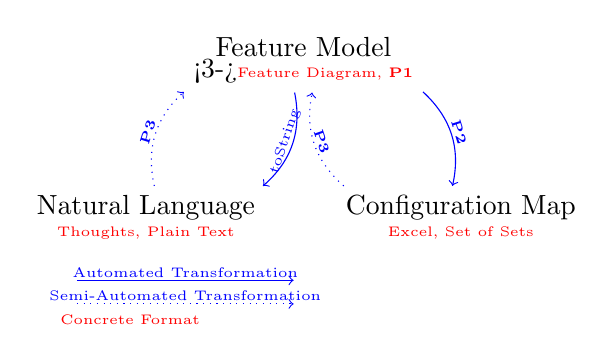
\begin{tikzpicture}
			\tikzstyle{every edge}=[font=\tiny,draw,color=blue]
			\node (fd) at (2,0) [align=center] {Feature Model\\[-1ex]{\uncover<3->{\tiny\color{red}Feature Diagram, \textbf{P1}}}};
			\node (nat) at (0,-2) [align=center] {Natural Language\\[-1ex]{\tiny\color{red}Thoughts, Plain Text}};
			\node (cfg) at (4,-2) [align=center] {Configuration Map\\[-1ex]{\tiny\color{red}Excel, Set of Sets}};

			\path [->] (fd) edge[bend left] node[sloped,yshift=1mm] {toString} (nat);
			\uncover<5->{\path [dotted, ->] (nat) edge[bend left] node[sloped,yshift=1mm] {\textbf{P3}} (fd);}
			
			\uncover<4->{\path [->] (fd) edge[bend left] node[sloped,yshift=1mm] {\textbf{P2}} (cfg);}
			\uncover<5->{\path [dotted, ->] (cfg) edge[bend left] node[sloped,yshift=1mm] {\textbf{P3}} (fd);}

			\node (trans) at (-1,-2.8) {};
			\node (trans2) at (2,-2.8) {};
			\node (trans3) at (-1,-3.1) {};
			\node (trans4) at (2,-3.1) {};
			\path [->] (trans) edge node[yshift=1mm] {Automated Transformation} (trans2);
			\path [dotted, ->] (trans3) edge[yshift=5mm] node[yshift=1mm] {Semi-Automated Transformation} (trans4);
		
			\node (bottomleft2) at (-0.2,-3.3) {\tiny\color{red}Concrete Format};
		\end{tikzpicture}

		\begin{note}{Problems}
			\begin{enumerate}
				\item<3->[P1] How to express feature models \emph{textually}?
				\item<4->[P2] How to (a) validate configurations and (b) get all valid configurations \emph{automatically}?
				\item<5->[P3] \color{gray}{(How to reverse engineer feature models?)}
			\end{enumerate}
		\end{note}
	\end{mycolumns}
\end{frame}

\subsection{UVL, the Universal Variability Language}

\begin{frame}[fragile]{\myframetitle\ \mytitlesource{\uvlwebsite}}
	\begin{mycolumns}
\begin{uvltight}[basicstyle=\normalsize]{}
features
	ConfigDB
		mandatory
			API {abstract}
				or
					Get
					Put
					Delete

		optional
			Transactions
		mandatory
			OS {abstract}
				alternative
					Windows
					Linux

constraints
	Transactions => Put | Delete
\end{uvltight}
	\mynextcolumn
		\begin{exampletight}{A Feature Model ``Sideways''}
			\centering
			\pic[width=\linewidth]{varied-model}
			$Transactions \pimplies Put \por Delete$
		\end{exampletight}
		\begin{note}{Universal Variability Language (UVL)}
			\begin{itemize}
				\item textual language for feature modeling
				\item adds advanced modeling constructs (e.g.,~attributes, cardinalities, submodels, \ldots)
			\end{itemize}
		\end{note}
	\end{mycolumns}
\end{frame}

\begin{frame}{Representations and Transformations}
	\begin{mycolumns}
		\centering
		\sffamily
		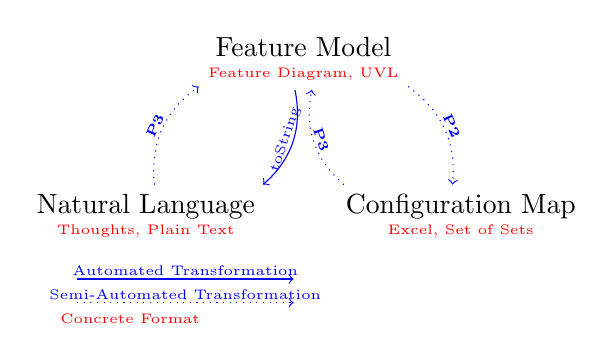
\begin{tikzpicture}
			\tikzstyle{every edge}=[font=\tiny,draw,color=blue]
			\node (fd) at (2,0) [align=center] {Feature Model\\[-1ex]{\tiny\color{red}Feature Diagram, UVL}};
			\node (nat) at (0,-2) [align=center] {Natural Language\\[-1ex]{\tiny\color{red}Thoughts, Plain Text}};
			\node (cfg) at (4,-2) [align=center] {Configuration Map\\[-1ex]{\tiny\color{red}Excel, Set of Sets}};

			\path [->] (fd) edge[bend left] node[sloped,yshift=1mm] {toString} (nat);
			\path [dotted, ->] (nat) edge[bend left] node[sloped,yshift=1mm] {\textbf{P3}} (fd);
			
			\path [dotted, ->] (fd) edge[bend left] node[sloped,yshift=1mm] {\textbf{P2}} (cfg);
			\path [dotted, ->] (cfg) edge[bend left] node[sloped,yshift=1mm] {\textbf{P3}} (fd);

			\node (trans) at (-1,-2.8) {};
			\node (trans2) at (2,-2.8) {};
			\node (trans3) at (-1,-3.1) {};
			\node (trans4) at (2,-3.1) {};
			\path [->] (trans) edge node[yshift=1mm] {Automated Transformation} (trans2);
			\path [dotted, ->] (trans3) edge[yshift=5mm] node[yshift=1mm] {Semi-Automated Transformation} (trans4);
		
			\node (bottomleft2) at (-0.2,-3.3) {\tiny\color{red}Concrete Format};
		\end{tikzpicture}
	\mynextcolumn
		\begin{note}{Problems}
			\begin{enumerate}
				\item[P1] How to express feature models \emph{textually}?
				\item[P2] How to (a) validate configurations and (b) get all valid configurations \emph{automatically}?
				\item[P3] \color{gray}{(How to reverse engineer feature models?)}
			\end{enumerate}
		\end{note}
		\begin{note}{Solutions}
			\begin{enumerate}
				\item[P1] Universal Variability Language $\Rightarrow$ \emph{Syntax}
				\item[P2] \emph{Semantics}?
				\item[P3] \color{gray}{--}
			\end{enumerate}
		\end{note}
	\end{mycolumns}
\end{frame}
% TODO first show the simpler version of the tikz picture, then animate towards the above, animate together with text
% TODO do we really need this slide? semantics was already defined in Part 4a for feature models

\subsection{Propositional Formulas}

\subsubsection*{Recap}

\begin{frame}{\myframetitle}
	\begin{mycolumns}
		\begin{definition}{Syntax of Propositional Formulas}
			Inductive definition of \emph{propositional formulas}\deutsch{\\aussagenlogische Formeln}:
			\begin{itemize}
				\item the \emph{Boolean truth values} $\top$, $\bot$
				\item any \emph{Boolean variable} $X$
    			\item any \emph{negation} $\pnot \phi$ of a formula $\phi$
    			\item any \emph{conjunction} $(\phi \pand \psi)$ of formulas $\phi$ and $\psi$
				\item any \emph{disjunction} $(\phi \por \psi)$, \emph{implication} $(\phi \pimplies \psi)$, or \emph{biimplication} $(\phi \pequals \psi)$
			\end{itemize}
		\end{definition}
	\mynextcolumn
		\begin{definition}{Informal Semantics of Propositional Formulas}
			\vspace*{-4ex}
			\begin{equation*}
				\begin{rcases}
					\top                \\
					\bot                \\
					\pnot \phi          \\
					\phi \pand \psi     \\
					\phi \por \psi      \\
					\phi \pimplies \psi \\
					\phi \pequals \psi
				\end{rcases} \text{ means } \begin{cases}
					\text{``true'' (or \emph{tautology})} \\
					\text{``false'' (or \emph{contradiction})} \\
					\text{``not $\phi$''} \\
					\text{``$\phi$ and $\psi$''} \\
					\text{``$\phi$ or $\psi$'' (inclusive or!)} \\
					\text{``if $\phi$, then $\psi$'' (and else?)} \\
					\text{``$\phi$ if and only if $\psi$''}
				\end{cases}
			\end{equation*}
		\end{definition}
		\begin{example}{Operator Precedence: $\pnot$, $\pand$, $\por$, $\pimplies$, $\pequals$}
			\vspace*{-4ex} % TODO Benno: why is this hack needed?
			\begin{align*}
				           &~Transactions \pimplies (Put \por Delete) \\
				\equiv     &~Transactions \pimplies Put \por Delete \\
				\not\equiv &~(Transactions \pimplies Put) \por Delete
			\end{align*}
		\end{example}
	\end{mycolumns}
\end{frame}

\subsubsection*{Example}

\begin{frame}{\myframetitle}
	\begin{mycolumns}[animation=none]
		\only<13|handout:2>{\addtocounter{framenumber}{+1}}\only<1-|handout:1-2>{
			\begin{exampletight}{A Feature Model $FM$ \ldots}
				\centering\tiny
				\featureDiagramConfigurableDatabase[_phi]
				\featureDiagramOverlay{
					\only<1|handout:0>{
						\featureDeemph{(API_phi),(Get_phi),(Put_phi),(Delete_phi),(Transactions_phi),(OS_phi),(Windows_phi),(Linux_phi)}
						\featureEmph{(ConfigDB_phi)}
					}
					\only<2|handout:0>{
						\featureDeemph{(Get_phi),(Put_phi),(Delete_phi),(Transactions_phi),(OS_phi),(Windows_phi),(Linux_phi)}
						\featureEmph{(ConfigDB_phi)(API_phi)}
					}
					\only<3|handout:0>{
						\featureDeemph{(Get_phi),(Put_phi),(Delete_phi),(API_phi),(OS_phi),(Windows_phi),(Linux_phi)}
						\featureEmph{(ConfigDB_phi)(Transactions_phi)}
					}
					\only<4|handout:0>{
						\featureDeemph{(Get_phi),(Put_phi),(Delete_phi),(API_phi),(Transactions_phi),(Windows_phi),(Linux_phi)}
						\featureEmph{(ConfigDB_phi)(OS_phi)}
					}
					\only<5|handout:0>{
						\featureDeemph{(ConfigDB_phi),(Transactions_phi),(Windows_phi),(Linux_phi),(OS_phi)}
						\featureEmph{(Get_phi)(Put_phi)(Delete_phi)(API_phi)}
					}
					\only<6-7|handout:0>{
						\featureDeemph{(Get_phi),(Put_phi),(Delete_phi),(API_phi),(Transactions_phi),(ConfigDB_phi)}
						\featureEmph{(Windows_phi)(Linux_phi)(OS_phi)}
					}
					\only<8|handout:0>{
						\featureDeemph{(ConfigDB_phi)(Transactions_phi)(Windows_phi)(Linux_phi)(OS_phi)(Get_phi)(Put_phi)(Delete_phi)(API_phi)}
					}
					\only<9-12|handout:1>{
						\featureSelected{(ConfigDB_phi),(API_phi),(Get_phi),(OS_phi),(Windows_phi)}
						\featureDeselected{(Put_phi)(Delete_phi),(Transactions_phi),(Linux_phi)}
					}
					\only<13-|handout:2>{
						\featureSelected{(ConfigDB_phi),(API_phi),(Get_phi)}
						\featureDeselected{(Put_phi)(Delete_phi)(Windows_phi)(Linux_phi),(Transactions_phi)(OS_phi)}
					}
				}
			\end{exampletight}
			\begin{exampletight}{\ldots as a Propositional Formula $\Phi(FM)$}
				\vspace*{-4ex}
				\small
				\begin{align*}
					\Phi(FM) = &~ConfigDB \\
					\uncover<2->{\pand &~(API \pequals ConfigDB) \\}
					\uncover<3->{\pand &~(Transactions \pimplies ConfigDB) \\}
					\uncover<4->{\pand &~(OS \pequals ConfigDB) \\}
					\uncover<5->{\pand &~(Get \por Put \por Delete \pequals API) \\}
					\uncover<6->{\pand &~(Windows \por Linux \pequals OS) \\}
					\uncover<7->{\pand &~\pnot (Windows \pand Linux) \\}
					\uncover<8->{\pand &~(Transactions \pimplies Put \por Delete)}
				\end{align*}
			\end{exampletight}
		}
	\mynextcolumn
		\only<9-|handout:1-2>{
			\begin{example}{Is This a Valid Configuration?}
				\vspace*{-4ex}
				\only<9-12|handout:1>{
					\begin{align*}
								&~\Phi(FM)({\{C, A, G, O, W\}}) \\
						\equiv	&~\Phi(FM)(\cfg[2-]{C, A, G, O, W}{P, D, T, L}) \\
						\uncover<10->{\equiv &~\fs{C} \pand (\fs{A} \pequals \fs{C}) \pand (\fd{T} \pimplies \fs{C}) \pand (\fs{O} \pequals \fs{C}) \\
								&~\pand (\fs{G} \por \fd{P} \por \fd{D} \pequals \fs{A}) \pand (\fs{W} \por \fd{L} \pequals \fs{O}) \\
								&~\pand \pnot (\fs{W} \pand \fd{L}) \pand (\fd{T} \pimplies \fd{P} \por \fd{D}) \\}
						\uncover<11->{\equiv &~\fs{\top} \pand (\fs{\top} \pequals \fs{\top}) \pand (\fd{\bot} \pimplies \fs{\top}) \pand (\fs{\top} \pequals \fs{\top}) \\
								&~\pand (\fs{\top} \por \fd{\bot} \por \fd{\bot} \pequals \fs{\top}) \pand (\fs{\top} \por \fd{\bot} \pequals \fs{\top}) \\
								&~\pand \pnot (\fs{\top} \pand \fd{\bot}) \pand (\fd{\bot} \pimplies \fd{\bot} \por \fd{\bot}) \\}
						\uncover<12->{\equiv &~\fs{\top} \pand \fs{\top} \pand \fs{\top} \pand \fs{\top} \pand \fs{\top} \pand \fs{\top} \pand \fs{\top} \pand \fs{\top} \\
						\equiv	&~\fs{\top}}
					\end{align*}
					\uncover<12->{\emph{$\leadsto$ configuration is valid}\\
					\phantom{$\leadsto$ }(read-only database on Windows)}
				}
				\only<13-|handout:2>{
					\begin{align*}
								&~\Phi(FM)({\{C, A, G\}}) \\
						\equiv	&~\Phi(FM)(\cfg[2-]{C, A, G}{P, D, T, O, W, L}) \\
						\uncover<14->{\equiv&~\fs{C} \pand (\fs{A} \pequals \fs{C}) \pand (\fd{T} \pimplies \fs{C}) \pand (\fd{O} \pequals \fs{C}) \\
								&~\pand (\fs{G} \por \fd{P} \por \fd{D} \pequals \fs{A}) \pand (\fd{W} \por \fd{L} \pequals \fd{O}) \\
								&~\pand \pnot (\fd{W} \pand \fd{L}) \pand (\fd{T} \pimplies \fd{P} \por \fd{D}) \\}
						\uncover<15->{\equiv&~\fs{\top} \pand (\fs{\top} \pequals \fs{\top}) \pand (\fd{\bot} \pimplies \fs{\top}) \pand (\fd{\bot} \pequals \fs{\top}) \\
								&~\pand (\fs{\top} \por \fd{\bot} \por \fd{\bot} \pequals \fs{\top}) \pand (\fd{\bot} \por \fd{\bot} \pequals \fd{\bot}) \\
								&~\pand \pnot (\fd{\bot} \pand \fd{\bot}) \pand (\fd{\bot} \pimplies \fd{\bot} \por \fd{\bot}) \\}
						\uncover<16->{\equiv&~\fs{\top} \pand \fs{\top} \pand \fs{\top} \pand \fd{\bot} \pand \fs{\top} \pand \fs{\top} \pand \fs{\top} \pand \fs{\top} \\
						\equiv	&~\fd{\bot}} % TODO: only show \pand and phi(fm) = and parentheses at the end
					\end{align*}
					\uncover<16->{\emph{$\leadsto$ configuration is invalid}\\
					\phantom{$\leadsto$ }($\lightning$ no operating system)}
				}
			\end{example}
		}
	\end{mycolumns}
\end{frame}

\subsubsection*{Algorithm}

\newcommand{\featureDiagramFn}[4]{#1\left(~\parbox{#2}{\centering\scalebox{0.8}{\featureDiagram{#3}}}~\right) &= #4}
\newcommand{\featureDiagramPhantom}[4]{\vphantom{#1\left(~\parbox{#2}{\centering\scalebox{0.8}{\featureDiagram{#3}}}~\right)}}

\begin{frame}{\myframetitle}
	\begin{mycolumns}[animation=none]
		\begin{definition}{Algorithm: Translate $FM$ Into $\Phi(FM)$}
			\begin{enumerate}
				\item<2-> translate each tree constraint
				\begin{itemize}
					\item<3-> \emph{Root feature}: $R$ is always required
						\item<4-> \emph{Optional feature}: $C$ requires $P$
						\item<5-> \emph{Mandatory feature}:\\
							Optional + $P$ requires $C$
						\item<6-> \emph{Or group}:\\
							Optional + $P$ requires at least one $C_i$
						\item<7-> \emph{Alternative group}:\\
							Optional + $P$ requires exactly one $C_i$
				\end{itemize}
				\item<8-> conjoin translated tree constraints\\
					$\Phi(TC) \gets \bigwedge_{tc \in TC} \Phi(tc)$
				\item<9-> conjoin \emph{cross-tree constraints}\\
					$\Phi(CTC) \gets \bigwedge_{ctc \in CTC} ctc$
				\item<10-> $\Phi(FM) \gets \Phi(TC) \pand \Phi(CTC)$
			\end{enumerate}
		\end{definition}
	\mynextcolumn
		\begin{definition}{}
			\vspace*{-4ex}
			\begin{align*}
				\uncover<3->{\featureDiagramFn{\Phi}{6ex}{Root,concrete}{Root}}\\
				\uncover<4->{\featureDiagramFn{\Phi}{6ex}{P,concrete[C,optional,concrete]}{C \pimplies P}}\\
				\uncover<5->{\featureDiagramFn{\Phi}{6ex}{P,concrete[C,mandatory,concrete]}{C \pequals P}}\\
				\uncover<6->{\featureDiagramFn{\Phi}{15ex}{P,concrete[$C_1$,or,concrete][\ldots,concrete][$C_n$,concrete]}{\bigvee_{1 \leq i \leq n} C_i \pequals P}}\\
				\uncover<7->{\featureDiagramFn{\Phi}{15ex}{P,concrete[$C_1$,alternative,concrete][\ldots,concrete][$C_n$,concrete]}{\bigvee_{1 \leq i \leq n} C_i \pequals P}}\\
				\uncover<7->{& \pand \bigwedge_{1 \leq i < j \leq n} \pnot (C_i \pand C_j)}
			\end{align*}
		\end{definition}
	\end{mycolumns}
\end{frame}

\subsection{CNF as a Universal Formula Language}

\begin{frame}{\myframetitle} % TODO unmotivated topic switch after prior slide?
	\begin{mycolumns}[animation=none]
		\begin{definition}{Recap: Conjunctive Normal Form}
			\begin{itemize}
				\item a \emph{literal} $L$ is a variable $X$ or its negation $\pnot X$
				\item a \emph{clause} $\clause{C}$ is a disjunction of literals $\clause{\bigvee_{j} L_j}$
				\item a \emph{conjunctive normal form (CNF)} is a conjunction of clauses $\bigwedge_{i} \clause{C_i} = \bigwedge_{i} \clause{\bigvee_{j} L_j}$
				\item intuitively: a set of ``rules'' to be satisfied
				\item any formula $\phi$ can be transformed into a CNF $\phi'$ that is logically equivalent ($\phi \mequals \phi'$)
			\end{itemize}
		\end{definition}
		\uncover<2->{
			\begin{definition}{Recap: Laws of Propositional Logic}
				\begin{itemize}
					\item<3-> implication: $\phi \pimplies \psi \mequals \pnot \phi \por \psi$
					\item<3-> biimplication: $\phi \pequals \psi \mequals (\pnot \phi \por \psi) \pand (\pnot \psi \por \phi)$
					\item<4-> De Morgan's laws: $\pnot (\phi \pand \psi) \mequals \pnot \phi \por \pnot \psi$
					\item<5-> distributivity:\,$(\phi \pand \psi) \por \chi \mequals (\phi \por \chi) \pand (\psi \por \chi)$
				\end{itemize}
			\end{definition}
		}
	\mynextcolumn
		\uncover<2->{
			\begin{example}{Transforming Part of $\Phi(FM)$ into $CNF(\Phi(FM))$}
				\vspace*{-4ex}
				\small
				% TODO: use color-blind friendly colors
				\begin{mycolumns}[animation=none]
					\begin{align*}
						\uncover<2->{&~\clause{C} \\
						\pand &~(T \pimplies C) \\
						\pand &~(O \pequals C) \\
						\pand &~(W \por L \pequals O) \\
						\pand &~\pnot (W \pand L)}
					\end{align*}
				\mynextcolumn
					\begin{align*}
						\uncover<3->{&~\clause{C} \\
						\pand &~\clause{(\pnot T \por C)} \\
						\pand &~\clause{(\pnot O \por C)} \pand \clause{(\pnot C \por O)} \\
						\pand &~(\pnot (W \por L) \por O) \\
						\pand &~\clause{(\pnot O \por W \por L)} \\
						\pand &~\pnot (W \pand L)}
					\end{align*}
				\end{mycolumns}
				\begin{mycolumns}[animation=none]
					\begin{align*}
						\uncover<4->{&~\clause{C} \\
						\pand &~\clause{(\pnot T \por C)} \\
						\pand &~\clause{(\pnot O \por C)} \pand \clause{(\pnot C \por O)} \\
						\pand &~((\pnot W \pand \pnot L) \por O) \\
						\pand &~\clause{(\pnot O \por W \por L)} \\
						\pand &~\clause{(\pnot W \por \pnot L)}}
					\end{align*}
				\mynextcolumn
					\begin{align*}
						\uncover<5->{&~\clause{C} \\
						\pand &~\clause{(\pnot T \por C)} \\
						\pand &~\clause{(\pnot O \por C)} \pand \clause{(\pnot C \por O)} \\
						\pand &~\clause{(\pnot W \por O)} \pand \clause{(\pnot L \por O)} \\
						\pand &~\clause{(\pnot O \por W \por L)} \\
						\pand &~\clause{(\pnot W \por \pnot L)}}
					\end{align*}
				\end{mycolumns}
			\end{example}
		}
	\end{mycolumns}
\end{frame} % TODO would be more intuitive to me if clauses are green (as they are good to go)

\subsubsection*{DIMACS}

\begin{frame}[fragile]{\myframetitle}
 	\begin{mycolumns}[columns=3,widths={25,25,50}]
		\vspace*{14ex}
		\begin{align*}
			&~C \\
			\pand &~(\pnot T \por C) \\
			\pand &~(\pnot O \por C) \pand (\pnot C \por O) \\
			\pand &~(\pnot W \por O) \pand (\pnot L \por O) \\
			\pand &~(\pnot O \por W \por L) \\
			\pand &~(\pnot W \por \pnot L)
		\end{align*}
 	\mynextcolumn
\begin{dimacstight}[basicstyle=\large]{}
c 1 C
c 2 T
c 3 O
c 4 W
c 5 L
p cnf 5 6
1 0
-2 1 0
-3 1 0 -1 3 0
-4 3 0 -5 3 0
-3 4 5 0
-4 5 0
\end{dimacstight}
	\mynextcolumn
		\begin{definition}{DIMACS Format\mysource{\dimacsformat}}
			\begin{itemize}
				\item de facto industry standard for storing CNF
				\item machine-readable, automated analyses, \ldots
				\item comments start with \texttt{c \ldots}
				\item problem line:\\
					\texttt{p cnf \#variables \#clauses}
				\item clause $\bigvee_{i} L_i$ translates to \texttt{L1 \ldots\ Ln 0}
				\item intuitively:
					\begin{equation*}
						\begin{rcases}
							\texttt{0}\\
							\texttt{\textvisiblespace}\\
							\texttt{-}
						\end{rcases} \text{ means } \begin{cases}
							\pand \\
							\por \\
							\pnot
						\end{cases}
					\end{equation*}
			\end{itemize}
		\end{definition}
 	\end{mycolumns}
\end{frame}

\begin{frame}{Representations and Transformations}
	\begin{mycolumns}[widths={52,48}]
		\centering
		\sffamily
		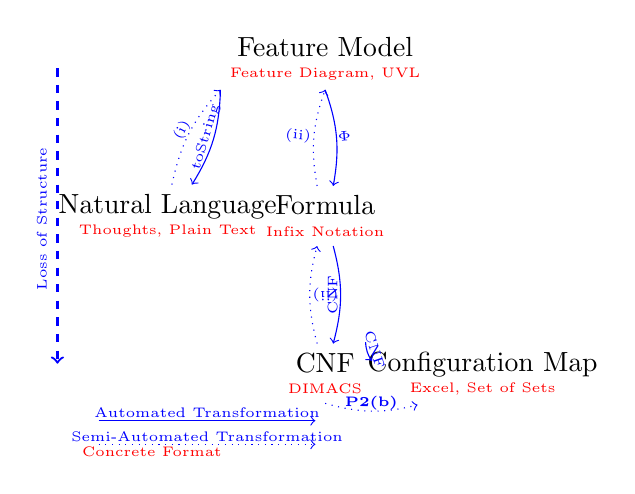
\begin{tikzpicture}
			\tikzstyle{every edge}=[font=\tiny,draw,color=blue]

			\node (topleft) at (-1.4,0) {};
			\node (bottomleft) at (-1.4,-4) {};
			
			\node (fd) at (2,0) [align=center] {Feature Model\\[-1ex]{\tiny\color{red}Feature Diagram, UVL}};
			\node (nat) at (0,-2) [align=center] {Natural Language\\[-1ex]{\tiny\color{red}Thoughts, Plain Text}};
			\node (phi) at (2,-2) [align=center] {Formula\\[-1ex]{\tiny\color{red}Infix Notation}};
			\node (cfg) at (4,-4) [align=center] {Configuration Map\\[-1ex]{\tiny\color{red}Excel, Set of Sets}};
			\node (cnf) at (2,-4) [align=center] {CNF\\[-1ex]{\tiny\color{red}DIMACS}};

			\path [dashed, thick, ->] (topleft) edge node[left, rotate=90, yshift=2mm, xshift=10mm] {Loss of Structure} (bottomleft);
		
			\path [->] (fd.south west) edge[bend left=15] node[sloped,yshift=1mm] {toString} (nat);
			\path [dotted, ->] (nat) edge[bend left=15] node[sloped,yshift=1mm] {(i)} (fd.south west);
			
			\path [->] (fd.south) edge[bend left=15] node[sloped,yshift=1mm,rotate=90] {$\Phi$} (phi);
			\path [dotted, ->] (phi) edge[bend left=15] node[sloped,yshift=2mm,rotate=270] {(ii)} (fd.south);

			\path [->] (phi) edge[bend left=15] node[sloped,yshift=1mm] {CNF} (cnf);
			\path [dotted, ->] (cnf) edge[bend left=15] node[sloped,yshift=2mm,rotate=270] {(ii)} (phi);
		
			\path [->] (cfg) edge[bend right=15] node[sloped,yshift=1mm] {CNF} (cnf);
			\path [dotted, ->] (cnf.south) edge[bend right=15] node[sloped,yshift=1mm] {\textbf{P2(b)}} (cfg);

			\node (trans) at (-1,-4.6) {};
			\node (trans2) at (2,-4.6) {};
			\node (trans3) at (-1,-4.9) {};
			\node (trans4) at (2,-4.9) {};
			\path [->] (trans) edge node[yshift=1mm] {Automated Transformation} (trans2);
			\path [dotted, ->] (trans3) edge[yshift=5mm] node[yshift=1mm] {Semi-Automated Transformation} (trans4);
		
			\node (bottomleft2) at (-0.2,-5) {\tiny\color{red}Concrete Format};
		\end{tikzpicture} % TODO would prefer another color for concrete formats, as they have nothing to do with the red boxes on thoses slides. what about green? needs to be changed consistently in all slides of this lecture
	\mynextcolumn
		\begin{note}{Problems}
			\begin{enumerate}
				\item[P1] How to express feature models \emph{textually}?
				\item[P2] How to 
				\begin{itemize}
					\item[(a)] validate configurations and
					\item[(b)] get all valid configurations
				\end{itemize}
				\emph{automatically}?
				\item[P3] \color{gray}{(How to reverse engineer feature models?)}
			\end{enumerate}
		\end{note}
		\begin{note}{Solutions}
			\begin{enumerate}
				\item[P1] Universal Variability Language $\Rightarrow$ \emph{Syntax}
				\item[P2] Propositional Formulas $\Rightarrow$ \emph{Semantics}
				\begin{itemize}
					\item[(a)] evaluate feature-model formula
					\item[(b)] \lecturemodeling\partc{}
				\end{itemize}
				\item[P3] \color{gray}{(i) e.g., \bakarnaturallanguage\\(ii) e.g., \czarneckithereandbackagain}
			\end{enumerate}
		\end{note}
	\end{mycolumns}
\end{frame}

% removed the following slide. could be confusing to use Excel in two different ways.
% \begin{frame}{\myframetitle}
% 	\centering
% 	\picDark[width=.8\linewidth,trim=10 10 0 10,clip]{constraints-in-excel}

% 	\textbf{``It's installed anyway.''}
% \end{frame}


\lessonslearned{
	\item to understand large configuration spaces, we need formal semantics and machine-readable representations
	\item propositional formulas satisfy many (though not all) needs for such a representation
}{
	\item Don Batory (2005): \href{https://doi.org/10.1007/11554844_3}{Feature Models, Grammars, and Propositional Formulas}
	\item Alexander Knüppel et al. (2017): \href{https://doi.org/10.1145/3106237.3106252}{Is There a Mismatch Between Real-World Feature Models and Product-Line Research?}
}{
	Translate the following feature diagram into a formula and then into CNF:

	\centering
	\featureDiagram{Root[A,optional[C,or][D]][B,mandatory[E,alternative][F]]}

	$D \pimplies E$
}

\sectionend

\section{Analyzing Feature Models}

\newcommand{\ssat}{\texttt{\#}SAT}
\usetikzlibrary{arrows,positioning}

\subsection{Configurators in the Wild}

\subsubsection*{Notebooks}

\begin{frame}{\myframetitle}
	\begin{mycolumns}[widths={70,30}]
		\myexampletight{Configuring a Notebook}{
			\only<1,3->{\pic[width=\linewidth]{thinkpad-x1-yoga-display}}\only<2|handout:0>{\pic[width=\linewidth]{thinkpad-x1-yoga-display-invalidconf}}
		}
	\mynextcolumn
		\mynote{}{
			can detect mistakes, but provides no explanations or fixes
		}
	\end{mycolumns}
\end{frame}

\begin{frame}{\myframetitle}
	\begin{mycolumns}[widths={70,30}]
		\myexampletight{Still Configuring a Notebook}{
			\pic[width=\linewidth]{thinkpad-x1-yoga-office}
		}
	\mynextcolumn
		\mynote{}{
			allows some feature combinations and not others, prices are opaque
		}
	\end{mycolumns}
\end{frame}

\subsubsection*{Cars}

\begin{frame}{\myframetitle}
	\begin{mycolumns}[widths={40,60},animation=none]
	\mynextcolumn
		\myexampletight{Configuring a Car}{
			\pic[width=\linewidth]{toyota-aygo-wheels}
		}
	\end{mycolumns}
\end{frame}

\begin{frame}{\myframetitle}
	\begin{mycolumns}[widths={40,60},reverse]
		\mynote{}{
			it is possible to create inconsistent states, leading to an invalid product
		}
	\mynextcolumn
		\myexampletight{Configuring a Car with a Weird Price}{
			\centering\pic[width=.55\linewidth]{toyota-aygo-costs}
		}
	\end{mycolumns}
\end{frame}

\begin{frame}{\myframetitle}
	\begin{mycolumns}[widths={40,60},reverse]
		\mynote{}{
			What happens if we ordered this \ldots?
		}
	\mynextcolumn
		\myexampletight{Configuring a Car with 8 Wheels!}{
			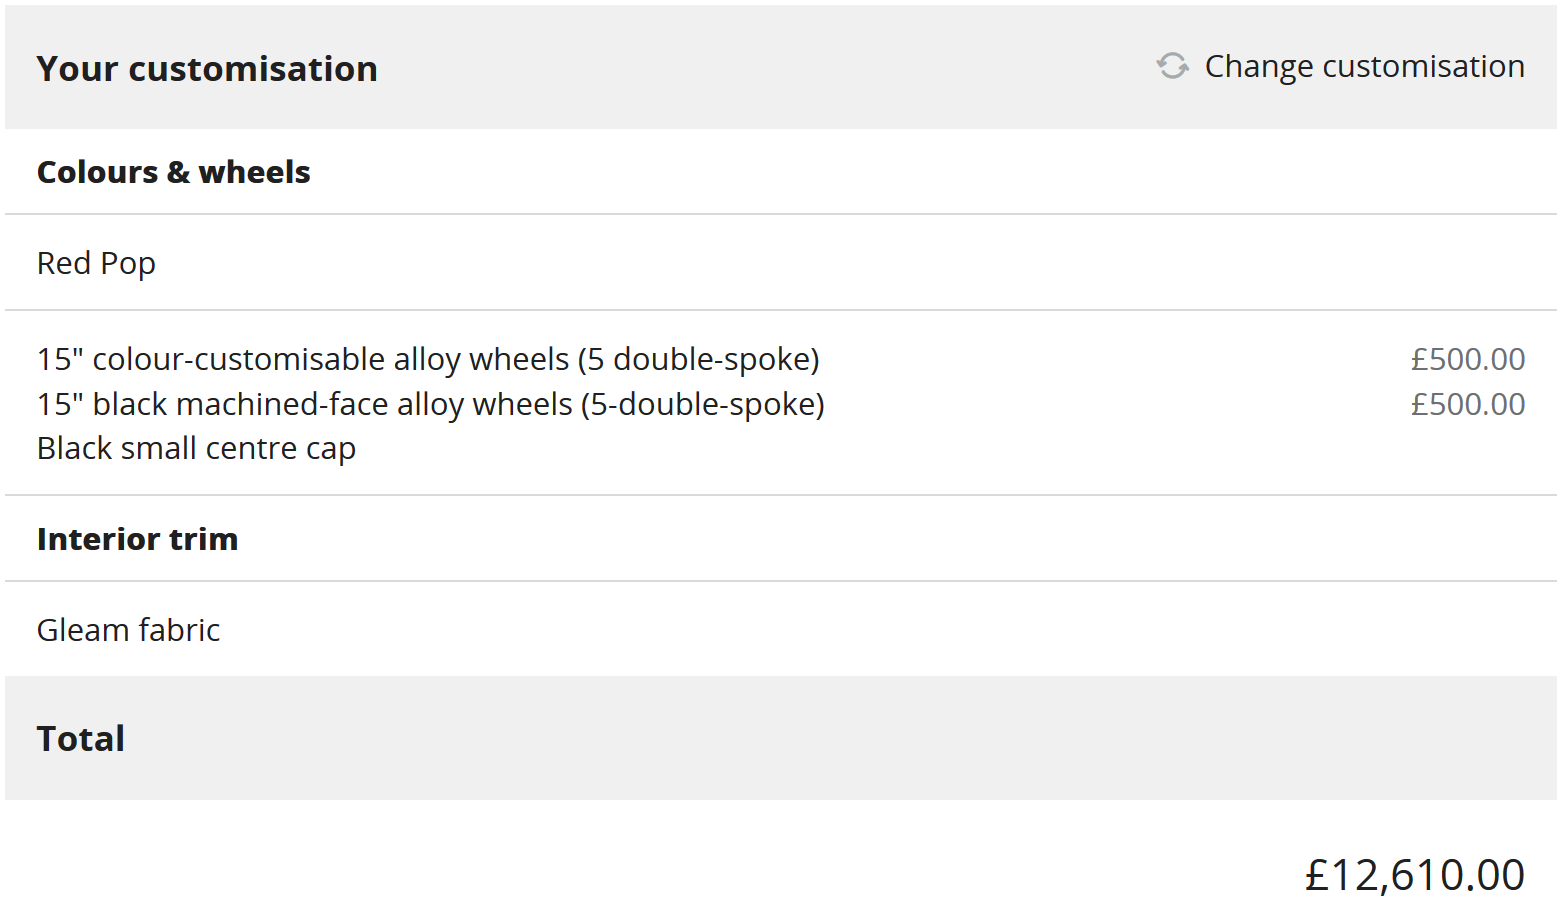
\includegraphics[width=\linewidth]{toyota-aygo-costs3}
		}
	\end{mycolumns}
\end{frame}

\begin{frame}{\myframetitle}
	\begin{mycolumns}[widths={70,30}]
		\myexampletight{Configuring a German Car}{
			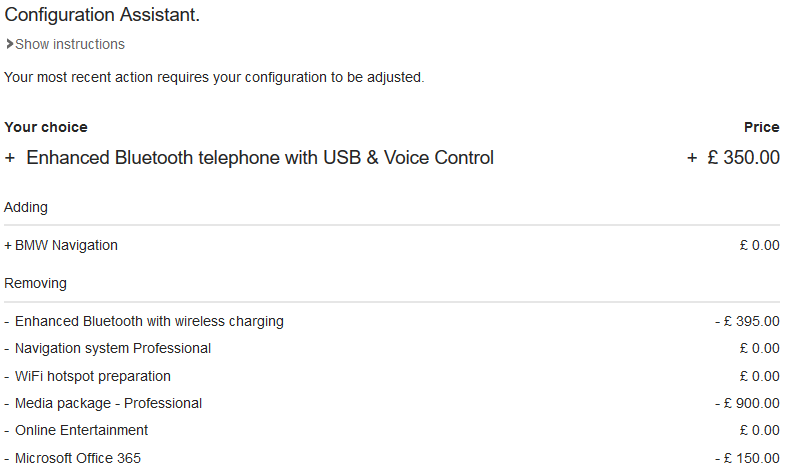
\includegraphics[width=\linewidth]{bmw-series1-confassistant-bluetooth}
		}
	\mynextcolumn
		\mynote{}{
			Why does the telephone conflict with Microsoft Office?
		}
	\end{mycolumns}
\end{frame}

\subsubsection*{Linux Kernel}

\begin{frame}{\myframetitle}
	\begin{mycolumns}[widths={60,40}]
		\myexampletight{}{
			\pic[width=\textwidth]{linux-menuconfig}
		}
	\mynextcolumn
		\mynote{make menuconfig}{
			\begin{itemize}
				\item configures KConfig models
				\item generates a \texttt{.config} file
				\item widely used to configure Linux
				\item still: it is possible to create invalid products
			\end{itemize}
		}
	\end{mycolumns}
\end{frame}

\subsection{Automated Analysis of Feature Models}

\begin{frame}{\myframetitle}
	\begin{mycolumns}
		\mynote{Open Questions}{
			\begin{itemize}
				\item How do such configurators work?
				\item How to avoid inconsistencies?
				\item How to provide explanations and fixes?
    			\item How to get all valid configurations automatically? (\emph{P2(b)})
			\end{itemize}
		}
		\mydefinition{Automated Analysis of Feature Models}{
			\begin{itemize}
				\item up until now: \emph{creation} and \emph{transformation} of feature models
				\item now: \emph{analysis} of feature models to improve our understanding of a configuration space
				\item for brevity: product = valid configuration
			\end{itemize}
		}
	\mynextcolumn
		\myexample{Asking Questions About Feature Models}{
			\begin{itemize}
				\item Is a given configuration valid?
				\item Is there any product at all?\\
					How many/which products are there?\\
				\item Is a given feature (de-)selectable at all?\\
					How many/which products include it?\\
				\item Is a given partial configuration consistent?\\
					How many/which products include it?\\
				\item \color{gray}{(Which features always occur together?)}
				\item \color{gray}{(Is a given constraint redundant?)}
				\item \color{gray}{(How do two feature model versions differ?)}
				\item \color{gray}{(Why is \ldots? How to fix \ldots?)}
			\end{itemize}
		}
	\end{mycolumns}
\end{frame}

\subsection{SAT, \ssat{}, and AllSAT Solvers}

\begin{frame}{\myframetitle}
	\begin{mycolumns}
		\mydefinition{Recap: Boolean Satisfiability Problem (SAT)}{
			\begin{itemize}
				\item \emph{decision problem}: is there any assignment that satisfies a given formula?
				\item formally: $SAT(\phi) \mequals \exists A \colon \phi(A) = \top$
				\item known to be \emph{NP-complete}:\\
					in theory, difficult to solve if $P \neq NP$;\\
					in practice, solvability depends on domain
				\item answered by \emph{SAT solvers}:\\
					highly-optimized, off-the-shelf tools;\\
					competitively developed over several decades;\\
					takes a CNF in DIMACS format as input
			\end{itemize}
		}
		\myexample{}{
			\begin{itemize}
				\item $X \pimplies Y$ is satisfiable
				\item $X \por \pnot X$ is satisfiable (even tautological)
				\item $X \pand \pnot X$ is not satisfiable (why?)
			\end{itemize}
		}
	\mynextcolumn
		\mydefinition{Sharp Satisfiability Problem (\ssat{})}{
			\begin{itemize}
				\item \emph{counting problem}: how many assignments satisfy a given formula?
				\item $\ssat(\phi) = \abs{\{A \mid \phi(A) = \top\}}$
				\item known to be \emph{\texttt{\#}P-complete}:\\
					at least as hard as SAT (probably harder)
				\item answered by \emph{\ssat{} solvers}
			\end{itemize}
		}
		\mydefinition{Solution Enumeration Problem (AllSAT)}{
			\begin{itemize}
				\item \emph{enumeration problem}: which assignments satisfy a given formula?
				\item $AllSAT(\phi) = \{A \mid \phi(A) = \top\}$
				\item at least as hard as \ssat{} (probably harder)
				\item answered by \emph{AllSAT solvers}
			\end{itemize}
		}
	\end{mycolumns}
\end{frame}

\begin{frame}{Automated Analysis of Feature Models}
	\begin{mycolumns}
		\myexample{Asking Questions About Feature Models}{
			\begin{itemize}
				\item Is a given configuration valid? $\Rightarrow$ \emph{evaluate}
				\item \emph{Is} there any valid configuration at all?\\
					\emph{How many}/\emph{which} valid configurations are there?\\
				\item \emph{Is} a given feature (de-)selectable at all?\\
					\emph{How many}/\emph{which} valid configurations include it?\\
				\item \emph{Is} a given partial configuration consistent?\\
					\emph{How many}/\emph{which} valid configurations include it?\\
			\end{itemize}
		}
		\mynote{Choosing the Right Solver}{
			\begin{itemize}
				\item ``is?''~~~~~~~~~~~~$\approx$ SAT solver query
				\item ``how many?''~$\approx$ \ssat{} solver query
				\item ``which?''~~~~~~\,$\approx$ AllSAT solver query
			\end{itemize}
		}
	\mynextcolumn
		\mydefinition{Typical Feature-Model Analysis Process}{
			\centering
			\begin{tikzpicture}
				\tikzset{block/.style={align=center,minimum height=5mm}}
				\node [block] (fm) {Feature Model};
				\node [block, right =4mm of fm] (formula) {Formula};
				\node [block, right =8mm of formula] (cnf) {DIMACS};
				\node [block, below right =8mm and -12mm of fm] (query) {Query};
				\node [block, right =10mm of query] (answer) {Answer};
				\node [block, right =12mm of answer] (result) {Result};
				\node [coordinate, below right =5mm and 2mm of cnf] (right) {};
				\node [coordinate, above left =3mm and 2mm of query] (left) {};
				\path[draw,->,color=blue] (fm) edge node[yshift=2mm] {\small $\Phi$} (formula)
							(formula) edge node[yshift=2mm] {\small $CNF$} (cnf)
							(cnf.east) -| (right) -- node[yshift=2mm] {\small formulate} (left) |- (query)
							(query) edge node[yshift=-2mm,align=center,font={\footnotesize}] {{\small solve}\\[1.5ex]SAT\\\ssat{}\\AllSAT} (answer)
							(answer) edge node [yshift=2mm]{\small interpret} (result);
			\end{tikzpicture}
		}
		\mynote{}{
			for brevity, we assume that $\phi = CNF(\Phi(FM))$ for a given feature model $FM$
		}
	\end{mycolumns}
\end{frame}

\subsection{Consistency, Cardinality, and Enumeration Queries}

\subsubsection{Feature Model}

\begin{frame}{\myframetitle}
	\begin{mycolumns}[t]
		\emph{Consistency of Feature Models (SAT)}
		\mydefinition{Void/Consistent Feature Model}{
			\begin{itemize}
				\item are there grave modeling errors?
				\item is it possible to configure any product at all?
			\end{itemize}
			\centering
			\begin{tikzpicture}
				\tikzset{block/.style={align=center,minimum height=5mm}}
				\node [block] (query) {$\phi$};
				\node [block, right =10mm of query] (answer) {$\bot/\top$};
				\node [block, above right =-3mm and 6mm of answer] (void) {$FM$ is \emph{void}};
				\node [block, below right =-3mm and 6mm of answer] (notvoid) {$FM$ is \emph{consistent}};
				\path[draw,->,color=blue] (query) edge node[yshift=2mm] {\small SAT} (answer)
							(answer) edge node [yshift=2mm,sloped]{\small $\bot$} (void)
							(answer) edge node [yshift=-2mm,sloped]{\small $\top$} (notvoid);
			\end{tikzpicture}
		}
		\mynextcolumn
		\emph{Cardinality of Feature Models (\ssat{})}
		\mydefinition{How Many Products Are There?}{
			\centering
			\begin{tikzpicture}
				\tikzset{block/.style={align=center,minimum height=5mm}}
				\node [block] (query) {$\phi$};
				\node [block, right =10mm of query] (answer) {$\abs{C}$};
				\path[draw,->,color=blue] (query) edge node[yshift=2mm] {\small \ssat{}} (answer);
			\end{tikzpicture}
		}
		\mydefinition{Variability Factor: Share of Products?}{
			\centering
			\begin{tikzpicture}
				\tikzset{block/.style={align=center,minimum height=5mm}}
				\node [block] (query) {$\phi$};
				\node [block, right =10mm of query] (answer) {$\abs{C}$};
				\node [block, right =6mm of answer] (num) {$\frac{\abs{C}}{2^{\abs{F}}}$};
				\path[draw,->,color=blue] (query) edge node[yshift=2mm] {\small \ssat{}} (answer)
							(answer) edge node [yshift=2mm,sloped]{} (num);
			\end{tikzpicture}
		}
	\end{mycolumns}
	\begin{mycolumns}[t]
		\myexampletight{}{
			\leftandright{
				\centering
				{\small\featureDiagram{Root,concrete[X,concrete,alternative][Y,concrete]}\\$\pnot (X \por Y)$}

				void
			}{
				\centering
				{\small\featureDiagram{Root,concrete[X,concrete,alternative][Y,concrete]}\\$X \por Y$}

				consistent
			}
		}
		\mynextcolumn
		\myexampletight{}{
			\leftandright{
				\centering
				{\small\featureDiagram{Root,concrete[X,concrete,alternative][Y,concrete]}\\$\pnot (X \por Y)$}

				$0$ products, VF $0$
			}{
				\centering
				{\small\featureDiagram{Root,concrete[X,concrete,alternative][Y,concrete]}\\$X \por Y$}

				$2$ products, VF $\frac{2}{8}$
			}
		}
	\end{mycolumns}
\end{frame}

\begin{frame}{\myframetitle}
	\begin{mycolumns}[t]
		\emph{Feasibility of SAT-Based Analyses}

		\mynote{Is Sat-Based Analysis ``Easy''?}{
			\begin{itemize}
				\item provocative claim: \mycite{SAT-based analysis of feature models is easy} \mysource{\href{https://dl.acm.org/doi/10.5555/1753235.1753267}{Mendonca~et~al.~2009}}
				\item easy $=$ performs much better than expected (although NP-complete)
				\item easy $=$ fast?
				\begin{itemize}
					\item what about formulating the query?\\
						(e.g., CNF transformation)
					\item what about many queries?\\
						(e.g., what we discuss next)
				\end{itemize}
			\end{itemize}
		}
	\mynextcolumn
		\emph{Feasibility of \ssat{}-Based Analyses}
	
		\myexampletight{Time to Count Products of Linux}{
			\includegraphics[width=\linewidth,page=4]{linux-plots}
		}
	\end{mycolumns}
\end{frame}


\begin{frame}{\myframetitle}
	\begin{mycolumns}
		\emph{Enumeration of Feature Models (AllSAT)}
		\mydefinition{Which Products Are There?}{
			\begin{itemize}
				\item \emph{P2(b)}: How to get all products?
			\end{itemize}
			\centering
			\begin{tikzpicture}
				\tikzset{block/.style={align=center,minimum height=5mm}}
				\node [block] (query) {$\phi$};
				\node [block, right =10mm of query] (answer) {$C$};
				\path[draw,->,color=blue] (query) edge node[yshift=2mm] {\small AllSAT} (answer);
			\end{tikzpicture}
		}
		\mynote{}{
			AllSAT does not scale to realistic feature models!\\
			50 features, configurations \`a 1 Byte $\approx$ 1 Petabyte
		}
		\myexampletight{}{
			\leftandright{
				\centering
				{\small\featureDiagram{Root,concrete[X,concrete,alternative][Y,concrete]}\\$\pnot (X \por Y)$}

				$\varnothing$
			}{
				\centering
				{\small\featureDiagram{Root,concrete[X,concrete,alternative][Y,concrete]}\\$X \por Y$}

				$\{\{Root, X\},\{Root, Y\}\}$
			}
		}
	\mynextcolumn
		\centering
		\sffamily
		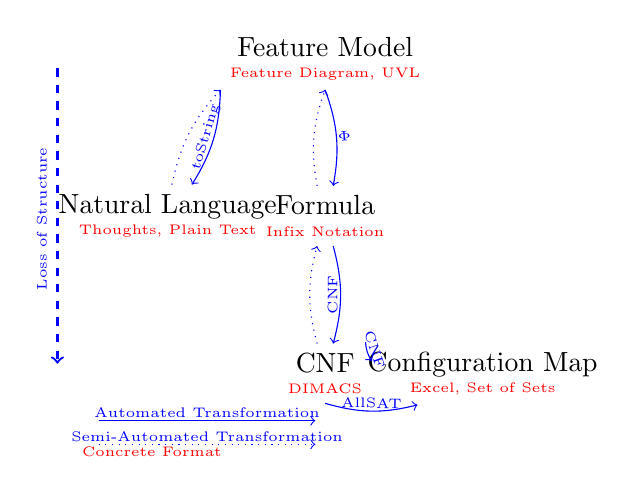
\begin{tikzpicture}
			\tikzstyle{every edge}=[font=\tiny,draw,color=blue]

			\node (topleft) at (-1.4,0) {};
			\node (bottomleft) at (-1.4,-4) {};
			
			\node (fd) at (2,0) [align=center] {Feature Model\\[-1ex]{\tiny\color{red}Feature Diagram, UVL}};
			\node (nat) at (0,-2) [align=center] {Natural Language\\[-1ex]{\tiny\color{red}Thoughts, Plain Text}};
			\node (phi) at (2,-2) [align=center] {Formula\\[-1ex]{\tiny\color{red}Infix Notation}};
			\node (cfg) at (4,-4) [align=center] {Configuration Map\\[-1ex]{\tiny\color{red}Excel, Set of Sets}};
			\node (cnf) at (2,-4) [align=center] {CNF\\[-1ex]{\tiny\color{red}DIMACS}};

			\path [dashed, thick, ->] (topleft) edge node[left, rotate=90, yshift=2mm, xshift=10mm] {Loss of Structure} (bottomleft);
		
			\path [->] (fd.south west) edge[bend left=15] node[sloped,yshift=1mm] {toString} (nat);
			\path [dotted, ->] (nat) edge[bend left=15] node[sloped,yshift=1mm] {} (fd.south west);
			
			\path [->] (fd.south) edge[bend left=15] node[sloped,yshift=1mm,rotate=90] {$\Phi$} (phi);
			\path [dotted, ->] (phi) edge[bend left=15] node[sloped,yshift=2mm,rotate=270] {} (fd.south);

			\path [->] (phi) edge[bend left=15] node[sloped,yshift=1mm] {CNF} (cnf);
			\path [dotted, ->] (cnf) edge[bend left=15] node[sloped,yshift=2mm,rotate=270] {} (phi);
		
			\path [->] (cfg) edge[bend right=15] node[sloped,yshift=1mm] {CNF} (cnf);
			\path [->] (cnf.south) edge[bend right=15] node[sloped,yshift=1mm] {AllSAT} (cfg);

			\node (trans) at (-1,-4.6) {};
			\node (trans2) at (2,-4.6) {};
			\node (trans3) at (-1,-4.9) {};
			\node (trans4) at (2,-4.9) {};
			\path [->] (trans) edge node[yshift=1mm] {Automated Transformation} (trans2);
			\path [dotted, ->] (trans3) edge[yshift=5mm] node[yshift=1mm] {Semi-Automated Transformation} (trans4);
		
			\node (bottomleft2) at (-0.2,-5) {\tiny\color{red}Concrete Format};
		\end{tikzpicture}
	\end{mycolumns}
\end{frame}

\subsubsection{Features}

\begin{frame}{\myframetitle}
	\begin{mycolumns}[t]
		\emph{Consistency of Features (SAT)}
		\mydefinition{Core/Dead Feature}{
			\begin{itemize}
				\item can a feature $F$ be (de-)selected at all?
			\end{itemize}
			\centering
			\begin{tikzpicture}
				\tikzset{block/.style={align=center,minimum height=5mm}}
				\node [block] (query) {$\phi \pand F$};
				\node [block, right =10mm of query] (answer) {$\bot/\top$};
				\node [block, above right =-3mm and 6mm of answer] (void) {$F$ is \emph{dead}};
				\node [block, below right =-3mm and 6mm of answer] (notvoid) {$F$ is not dead};
				\path[draw,->,color=blue] (query) edge node[yshift=2mm] {\small SAT} (answer)
							(answer) edge node [yshift=2mm,sloped]{\small $\bot$} (void)
							(answer) edge node [yshift=-2mm,sloped]{\small $\top$} (notvoid);
			\end{tikzpicture}
			\begin{tikzpicture}
				\tikzset{block/.style={align=center,minimum height=5mm}}
				\node [block] (query) {$\phi \pand \pnot F$};
				\node [block, right =10mm of query] (answer) {$\bot/\top$};
				\node [block, above right =-3mm and 6mm of answer] (void) {$F$ is \emph{core}};
				\node [block, below right =-3mm and 6mm of answer] (notvoid) {$F$ is not core};
				\path[draw,->,color=blue] (query) edge node[yshift=2mm] {\small SAT} (answer)
							(answer) edge node [yshift=2mm,sloped]{\small $\bot$} (void)
							(answer) edge node [yshift=-2mm,sloped]{\small $\top$} (notvoid);
			\end{tikzpicture}
		}
		\mynextcolumn
		\emph{Cardinality of Features (\ssat{})}
		\mydefinition{How Many Products Include Feature $F$?}{
			\centering
			\begin{tikzpicture}
				\tikzset{block/.style={align=center,minimum height=5mm}}
				\node [block] (query) {$\phi \pand F$};
				\node [block, right =10mm of query] (answer) {$\abs{\{S \in C \mid F \in S\}}$};
				\path[draw,->,color=blue] (query) edge node[yshift=2mm] {\small \ssat{}} (answer);
			\end{tikzpicture}
		}
		\mydefinition{Commonality: How Dead is This Feature?}{
			\centering
			\begin{tikzpicture}
				\tikzset{block/.style={align=center,minimum height=5mm}}
				\node [block] (query) {$\phi \pand F$};
				\node [block, right =7mm of query] (answer) {$\abs{\{S \in C \mid F \in S\}}$};
				\node [block, right =2mm of answer] (num) {$\frac{\abs{\{S \in C \mid F \in S\}}}{\abs{C}}$};
				\path[draw,->,color=blue] (query) edge node[yshift=2mm] {\small \ssat{}} (answer)
							(answer) edge node [yshift=2mm,sloped]{} (num);
			\end{tikzpicture}
		}
	\end{mycolumns}
	\begin{mycolumns}[t]
		\myexampletight{}{
			\centering
			{\small\featureDiagram{Root,concrete[X,concrete,alternative][Y,concrete]}\\$\pnot X$}

			$X$ is dead, $Root$ and $Y$ are core
		}
		\mynextcolumn
		\myexampletight{}{
			\centering
			{\small\featureDiagram{Root,concrete[X,concrete,alternative][Y,concrete]}\\$\pnot X$}

			$X$: 0 products, $Root$ and $Y$: 1 products
		}
	\end{mycolumns}
\end{frame}

\subsubsection{Partial Configurations}

\begin{frame}{\myframetitle}
	\begin{mycolumns}[t]
		\emph{Consistency of Partial Configurations (SAT)}
		\mydefinition{Valid Partial Configuration}{
			\begin{itemize}
				\item does a partial configuration $C = ({\color{green}S}, {\color{red}D})$ contain a mistake?
			\end{itemize}
			\centering
			\begin{tikzpicture}
				\tikzset{block/.style={align=center,minimum height=5mm}}
				\node [block] (query) {$\phi \pand \bigwedge_{s \in S} {\color{green}s} \pand \bigwedge_{d \in D} {\color{red}\pnot d}$};
				\node [block, right =10mm of query] (answer) {$\bot/\top$};
				\node [block, above right =-3mm and 6mm of answer] (void) {$C$ $\times$};
				\node [block, below right =-3mm and 6mm of answer] (notvoid) {$C$ \checkmark};
				\path[draw,->,color=blue] (query) edge node[yshift=2mm] {\small SAT} (answer)
							(answer) edge node [yshift=2mm,sloped]{\small $\bot$} (void)
							(answer) edge node [yshift=-2mm,sloped]{\small $\top$} (notvoid);
			\end{tikzpicture}
		}
		\mynextcolumn
		\emph{Cardinality of Partial Configurations (\ssat{})}
		\mydefinition{How Many Products Are Still Configurable for $C$?}{
			\centering
			\begin{tikzpicture}
				\tikzset{block/.style={align=center,minimum height=5mm}}
				\node [block] (query) {$\phi \pand ...$};
				\node [block, right =10mm of query] (answer) {$\abs{\{(S', D') \in C \mid {\color{green}S} \subseteq S', {\color{red}D} \in D'\}}$};
				\path[draw,->,color=blue] (query) edge node[yshift=2mm] {\small \ssat{}} (answer);
			\end{tikzpicture}
		}
	\end{mycolumns}
	\begin{mycolumns}[t]
		\myexampletight{}{
			\centering
			{\small\featureDiagram{Root,concrete[X,concrete,optional][Y,concrete,optional]}\\$X \pimplies Y$}

			\cfg{Root}{X} \checkmark
		}
		\mynextcolumn
		\myexampletight{}{
			\centering
			{\small\featureDiagram{Root,concrete[X,concrete,optional][Y,concrete,optional]}\\$X \pimplies Y$}

			\cfg{Root}{X}: 2 products
		}
	\end{mycolumns}
\end{frame}

\subsection{Automated Analyses in FeatureIDE}

\subsubsection*{Feature-Model Editor}

\begin{frame}{\myframetitle}
	\begin{mycolumns}[widths={60,40}]
		\myexampletight{}{
			\pic[width=\textwidth]{featureide-feature-model-editor-waffle}
		}
	\mynextcolumn
		\myexampletight{}{
			\pic[width=\textwidth]{featureide-feature-model-statistics}
		}
	\end{mycolumns}
\end{frame}

\subsubsection*{Configuration Editor}

\begin{frame}{\myframetitle}
	\begin{mycolumns}[widths={60,40}]
		\myexampletight{}{
			\centering
			\pic[width=.27\textwidth]{featureide-configuration-editor-step1}
			$\Rightarrow$
			\pic[width=.63\textwidth]{featureide-configuration-editor-step2}
		}
	\mynextcolumn
		\mynote{Decision Propagation}{
			\begin{itemize}
				\item after each decision (i.e., click) \ldots
				\begin{itemize}
					\item \ldots{} select features that are now \emph{conditionally core}
					\item \ldots{} deselect features that are now \emph{conditionally dead}
				\end{itemize}
				\item this way it is impossible to configure an invalid product
				\item explanations for all propagated decisions
			\end{itemize}
		}
	\end{mycolumns}
\end{frame}

\begin{frame}{Automated Analysis of Feature Models}
	\begin{mycolumns}
		\mydefinition{The Road So Far \ldots}{
			\centering
			\begin{tikzpicture}
				\tikzset{block/.style={align=center,minimum height=5mm}}
				\node [block] (fm) {Feature Model};
				\node [block, right =4mm of fm] (formula) {Formula};
				\node [block, right =8mm of formula] (cnf) {DIMACS};
				\node [block, below right =8mm and -12mm of fm] (query) {Query};
				\node [block, below =-.5mm of query,align=center,color=blue,font={\footnotesize}] (query2) {void feature model\\variability factor\\all products\\core/dead features\\false-optional features\\commonality\\valid partial configuration\\decision propagation};
				\node [block, right =27mm of query] (answer) {Answer};
				\node [block, right =4mm of answer] (result) {};
				\node [coordinate, below right =5mm and 2mm of cnf] (right) {};
				\node [coordinate, above left =3mm and 2mm of query] (left) {};
				\path[draw,->,color=blue] (fm) edge node[yshift=2mm] {\small $\Phi$} (formula)
							(formula) edge node[yshift=2mm,align=center] {\small $CNF$} (cnf)
							(cnf.east) -| (right) -- node[yshift=2mm] {\small formulate} (left) |- (query)
							(query) edge node[yshift=-2mm,align=center,font={\footnotesize}] {{\small solve}\\[1.5ex]SAT\\\ssat{}\\AllSAT} (answer)
							(answer) edge (result);
			\end{tikzpicture}
		}
	\mynextcolumn
		\mydefinition{\ldots and Beyond}{
			\centering
			\begin{tikzpicture}
				\tikzset{block/.style={align=center,minimum height=5mm}}
				\node [block,align=center,color=red,font={\footnotesize}] (fm2) {attributes\\cardinalities\\submodels};
				\node [block, below =.5mm of fm2] (fm) {Feature Model};
				\node [block, right =4mm of fm] (formula) {Formula};
				\node [block, above =.5mm of formula,align=center,color=red,font={\footnotesize}] (formula2) {quantifiers\\predicates\\functions};
				\node [block, right =8mm of formula] (cnf) {DIMACS};
				\node [block, above =.5mm of cnf,align=center,color=red,font={\footnotesize}] (cnf2) {DNF\\d-DNNF\\BDD};
				\node [block, below right =8mm and -12mm of fm] (query) {Query};
				\node [block, below =-.5mm of query,align=center,color=red,font={\footnotesize}] (query2) {atomic sets\\redundant constraints\\feature-model edits\\explanations\\sampling\\slicing};
				\node [block, right =27mm of query] (answer) {Answer};
				\node [block, right =4mm of answer] (result) {};
				\node [coordinate, below right =5mm and 2mm of cnf] (right) {};
				\node [coordinate, above left =3mm and 2mm of query] (left) {};
				\path[draw,->,color=blue] (fm) edge node[yshift=2mm] {\small $\Phi$} (formula)
							(formula) edge node[yshift=0mm,align=center] {\small $CNF$\\{\footnotesize\color{red}Tseitin}} (cnf)
							(cnf.east) -| (right) -- node[yshift=2mm] {\small formulate} (left) |- (query)
							(query) edge node[yshift=-7mm,align=center,font={\footnotesize}] {{\small solve}\\[1.5ex]SAT, \ssat{}, AllSAT\\{\color{red}MAX-SAT}\\{\color{red}Solution-SAT}\\{\color{red}MUS}\\{\color{red}SMT, CSP}\\{\color{red}QBF}\\{\color{red}WMC, PMC}} (answer)
							(answer) edge (result);
			\end{tikzpicture}
			\vspace*{-4ex}
			\begin{itemize}
				\item develop new analyses
				\item improve efficiency of existing analyses
				\item investigate correctness and compositionality
			\end{itemize}
		}
	\end{mycolumns}
\end{frame}

\lessonslearned{
	\item with solvers, we can build reliable configurators for product lines
	\item SAT-based analyses: void feature model, core/dead features, decision propagation
	\item \ssat{}-based analyses: variability factor, feature commonality
}{
	\item \fospl, Section~10.1 Analysis of Feature Models
	\item David Benavides et al. (2010): \href{https://doi.org/10.1016/j.is.2010.01.001}{Automated Analysis of Feature Models 20 Years Later: A Literature Review}
	\item Chico Sundermann et al. (2021): \href{https://doi.org/10.1145/3442391.3442404}{Applications of \#SAT Solvers on Feature Models}
}{
	Consider this feature diagram:

	\begin{center}
		\featureDiagram{Root[A,optional[C,or][D]][B,mandatory[E,alternative][F]]}
	\end{center}

	How can you \ldots
	\begin{itemize}
		\item make this feature model void
		\item make exactly one feature dead
	\end{itemize}
	\ldots{} by adding one constraint, respectively?

	Name a partial configuration for which only two products exist.
}

\mode<beamer>{
	\begin{frame}{\inserttitle}
		\lectureseriesoverview
	\end{frame}

	\contentoverview
}


\end{document}
